{\fontsize{12pt}{22pt} \textbf{Performance metrics for classification}\par}

\vspace{5mm}

1) ROC = Receiver Operating Curve \\

\underline{Use of the ROC}

\vspace{5mm}

One model:

We use the ROC to evaluate the performance of one classifying model that we can obtain when varying a threshold.

\vspace{5mm}

Several models:

We use the ROC to compare several classifying models in evaluating the area under the curve (AUC) for a range of threshold.

\vspace{5mm}

\underline{Intuition}

\vspace{5mm}

After running the prediction of a specific model, we draw the confusion matrix (actual vs predited) with a certain threshold.

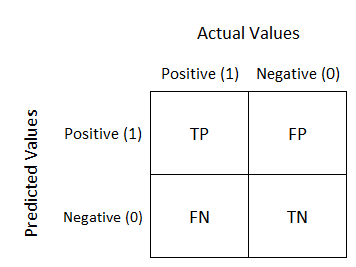
\includegraphics[scale=0.5]{confusionmatrice.png}

\vspace{5mm}

We then modify the threshold and draw another confusion matrix.

The ROC summarizes all of the confusion matrices that each threshold produced.

\vspace{5mm}

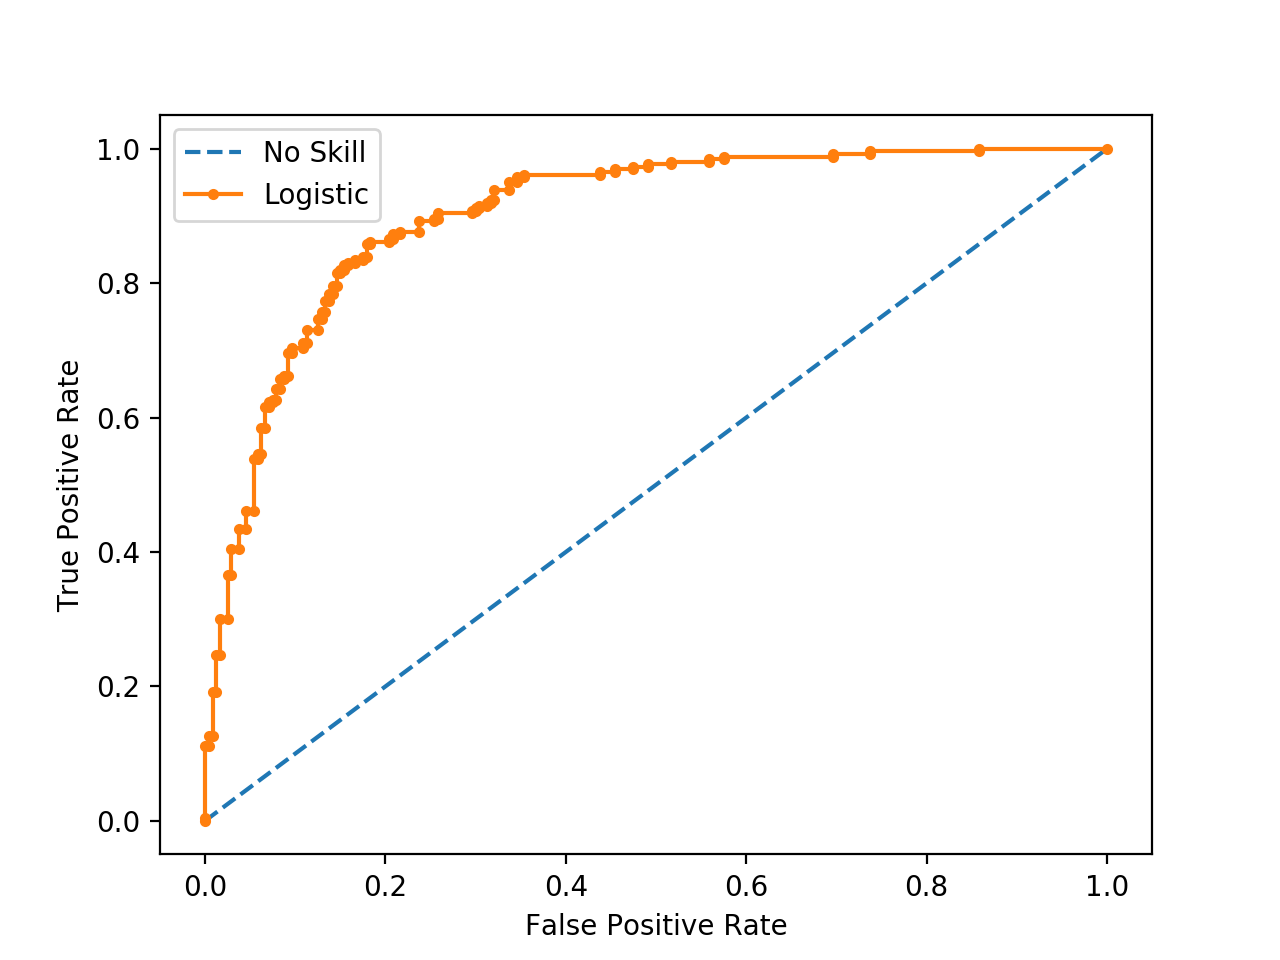
\includegraphics[scale=0.5]{ROC.png}

\vspace{5mm}

The curve is drawn using relationship ratios between predictions and actual results: \\

X-axis: $$FPR = \frac{FP}{N} = \frac{FP}{FP + TN}$$

Y-axis: $$TPR = \frac{TP}{P} = \frac{TP}{TP + FN}$$

\vspace{5mm}

\underline{Implementation}

\vspace{5mm}

1. Get probability predictions

2. Sort the probabilities (prediction)

3. Sort the validation (actual) according to previous sort

4. Loop on the sorted validation. At each iteration:

- increment TP or FP

- compute the TPR and FPR.

5. Plot (FPR, TPR)

\vspace{5mm}

See \textit{https://docs.eyesopen.com/toolkits/cookbook/python/plotting/roc.html} for an implementation example, or data challenge Face\_Recognition. \\

2) PR curve = Precision-Recall curve \\

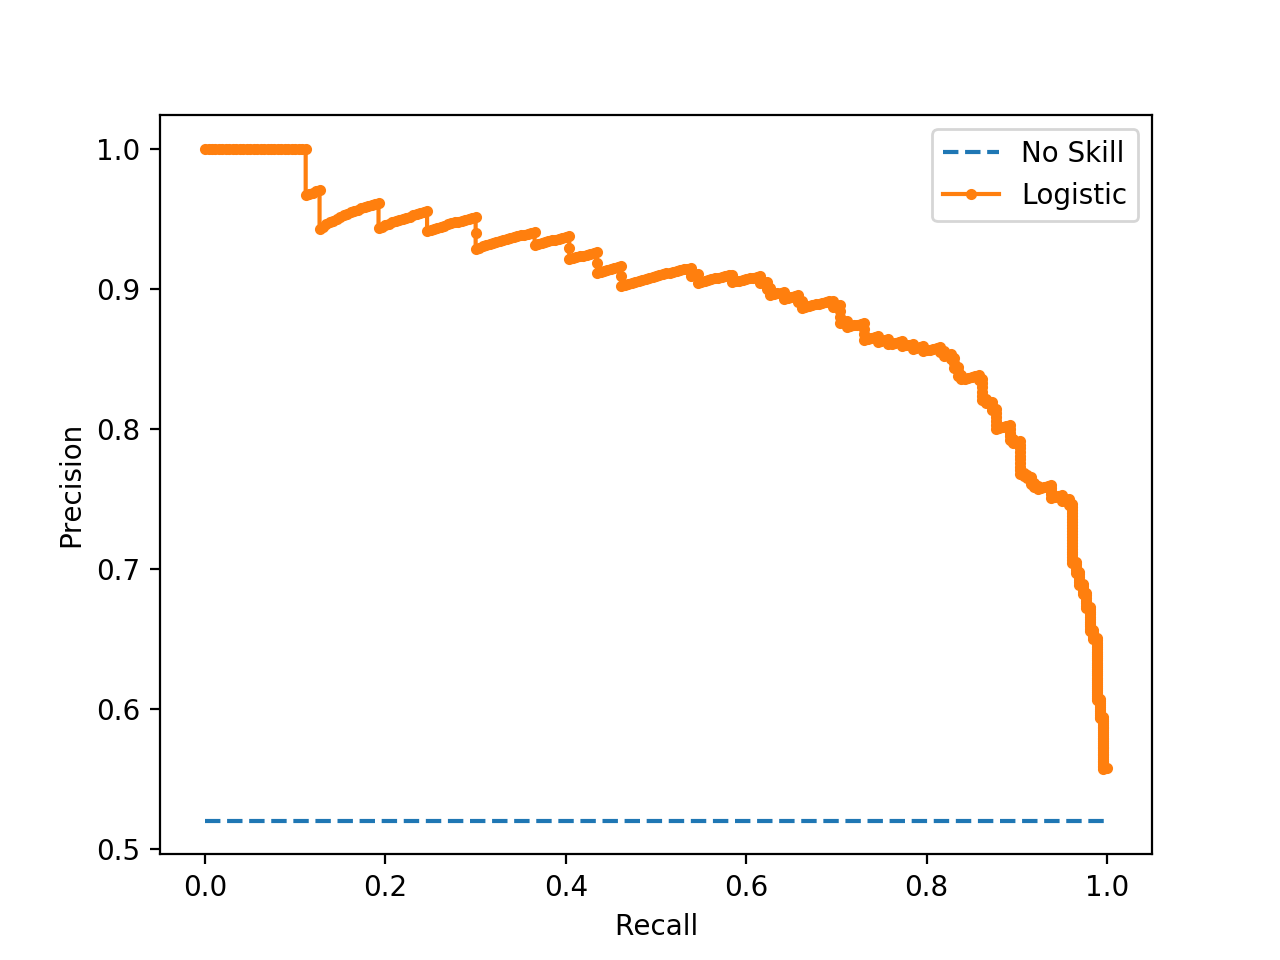
\includegraphics[scale=0.5]{PR_curve.png}

The PR curve uses the following ratios: \\

X-axis:

$$\text{Recall} = TPR = \frac{TP}{P} = \frac{TP}{TP + FN}$$

Y-axis:

$$\text{Precision} = \frac{TP}{TP + FP}$$ \\

The PR curve is better adapted than the ROC in the case of imbalanced data: \\

ROC uses $FPR = \frac{FP}{\textcolor{red}{N}} $ --> $N$ can be either very large or very small if classes are imbalanced.

PR curve uses $\text{Precision} = \frac{TP}{\textcolor{green}{TP + FP}}$ --> the precision considers only the positive values coming from the model.



\vspace{5mm}
